\chapter{Methodology}
\label{ch:method}

\section{Data Collection and Preprocessing}

\subsection{Data Sources}

\begin{itemize}
    \item \textbf{Database of East African Mesoscale Convective Systems (MCSs)}
    \begin{itemize}
        \item File: \texttt{East\_Africa\_tracked\_MCSs\_2014\_2019\_longer\_than\_3\_hours.csv}
        \item Contains 27,982 storms longer than 3 hours, with all storm centroids along the track within (3--15N, 34--52E)
    \end{itemize}
    \item \textbf{ERA5 Data}
    \begin{itemize}
        \item ERA5 data for 31--53E, 2--16N region for 2014--2019, totalling 27 GB
        \item The ERA5 area is slightly wider by a few grid points to account for edge cases in the database and for calculating gradients
    \end{itemize}
\end{itemize}

\subsection{Feature Engineering}

\begin{itemize}
    \item cleaning
    \item means over 400km
    \item domain means
    \item storm aggregate features
\end{itemize}

\subsection{Feature Selection}

\begin{itemize}
    \item highly correlated features removed
    \item data leakage prevention measures implemented
    \begin{itemize}
        \item related features
        \item features with info from future
    \end{itemize}
\end{itemize}

\section{Modelling Approach}

The following section describes the \acrshort{ml} approach taken to predict storm intensification and propagation. As all predictands are continuous variables and the input features can be directly associated with the target storm characteristics, this \acrshort{ml} task is classified as supervised regression as opposed to unsupervised learning, where the target variables are not known, or classification, where the goal is to predict discrete labels.

\subsection{XGBoost}

In this thesis, \acrfull{xgb} is the modelling framework employed for this supervised regression task. In part, the decision to use \acrshort{xgb} corresponds with faithfully reproducing the methodology of \cite{Hunt2024}. However, their choice is justified by the advantages that the approach presents. \acrshort{xgb} is a decision-tree based model leveraging an efficient and scalable implementation of gradient boosting \citep{Chen2016}. Gradient boosting, an extension of \gls{ensemblelearning}, iteratively trains weak learners, in this case decision trees, on the residual errors of the previous learners. This process allows the model to focus on the most challenging examples to improve overall performance while also preventing overfitting, especially when compared to one, highly complex decision tree model \citep{Friedman2001}. Yet, since the model retains its underlying structure of decision trees, it remains directly interpretable through techniques like feature importance. Generally, feature importance is a global model-agnostic \acrshort{xai} method that quantifies the contribution of each feature to the model's predictions by measuring the change in the model's performance when the feature is permuted \citep{Musolf2022}. In decision-tree based models, the nature of the trees themselves can be exploited to more efficiently calculate importance. Typically, this is based on metrics like the frequency with which a feature is used for splitting, the average gain in accuracy from splits involving that feature, or the total reduction in impurity attributed to that feature across all trees in the ensemble \citep{Louppe2013}. Although not used in this thesis, the inherent interpretability of \acrshort{xgb} through feature importance analysis aligns with the goals of this research.

\subsection{Hyperparameter Tuning}

\acrshort{xgb} provides a myriad of hyperparameters that can be adjusted to optimise model performance. These include parameters controlling the learning rate, tree depth, number of trees, and regularisation terms, among others. The choice of hyperparameters can significantly impact the model's ability to generalise to unseen data. Therefore, a systematic approach to hyperparameter tuning is essential. In this thesis, hyperparameter tuning is conducted using \acrfull{wandb}, a popular web-based tool for tracking and visualising \acrshort{ml} experiments \insertref{wandb}. Specifically, a sweep with Bayesian optimisation is employed to efficiently explore the hyperparameter space and identify optimal configurations. Bayesian optimisation is particularly well-suited for this task as it builds a probabilistic model of the objective function and uses it to select the most promising hyperparameters to evaluate next \insertref{bayes opt}\todo{better desc/wording}. This approach balances exploration and exploitation, allowing for a more efficient search compared to grid or random search methods \insertref{probably same as last one}.

Additionally, cross-validation is utilised during training on each trial to ensure that the model's performance is robust and not overly dependent on a specific subset of the data. Specifically, the dataset is first split into a training set and a test set to ensure that some data remains completely unseen throughout the training process. Then, within the training set, k-fold cross-validation is applied, where the dataset is divided into k subsets and the model is trained and validated k times, each time using a different subset as the validation set and the remaining subsets for training. Once all folds are complete, the best performing model is chosen as the result of the trial. This method provides a more reliable estimate of model performance on the given hyperparameters \insertref{cross val performance}\todo{better desc/wording}.

The specific hyperparameters tuned and the corresponding values or distributions used for the sweep are included in Table \ref{tab:wandb-sweep-config}. The remaining hyperparameters were kept at their default values as defined in the \acrshort{xgb} Python implementation \insertref{need a link to xgb docs here?}.

\begin{table}[!ht]
    \centering
    \caption{\acrshort{wandb} Sweep Configuration for \acrshort{xgb} Hyperparameter Tuning. The names in this table refer to the hyperparameter names for the Scikit-Learn wrapper interface for \acrshort{xgb}. A full description of each hyperparameter can be found in the \href{https://xgboost.readthedocs.io/en/stable/python/python_api.html\#module-xgboost.sklearn}{XGBoost documentation}.}
    \label{tab:wandb-sweep-config}
    \begin{tabular}{llr}     
        \toprule
        \textbf{Hyperparameter} & \textbf{Values / Distribution} \\ 
        \midrule
        Gamma ($\gamma$) & Uniform[0, 5] \\
        Regularisation Alpha ($\alpha$) & Uniform[0, 5] \\
        Regularisation Lambda ($\lambda$) & Uniform[0, 5] \\
        Column Subsample by Tree & Uniform[0, 1.0] \\
        Learning Rate & Uniform[0, 1.0] \\
        Max Depth & \{3, 6, 9, 12\} \\
        Number of Estimators & \{60, 120, 180\} \\
        \bottomrule
    \end{tabular}
\end{table}

\subsection{Performance Comparison}

\begin{itemize}
    \item compare performance metrics test RMSE across different models
    \item analyse discrepancies in performance across different feature sets
    \item analyse average performance across different regions and time periods? \todo{if no time, this is for future work section}
\end{itemize}

\section{Model Explainability}
\todo{copied from background; will need to be adapted}

\acrfull{xai} is an emerging field focused on developing methods and techniques to make the decision-making processes of \acrshort{ml} solutions more transparent and interpretable. Approaches in this field take a variety of forms, including inherently interpretable models and post-hoc explanation methods. A summary of \acrshort{xai} taxonomy is given in Figure \ref{fig:xai-taxonomy}.

\begin{figure}[ht]
    \centering
    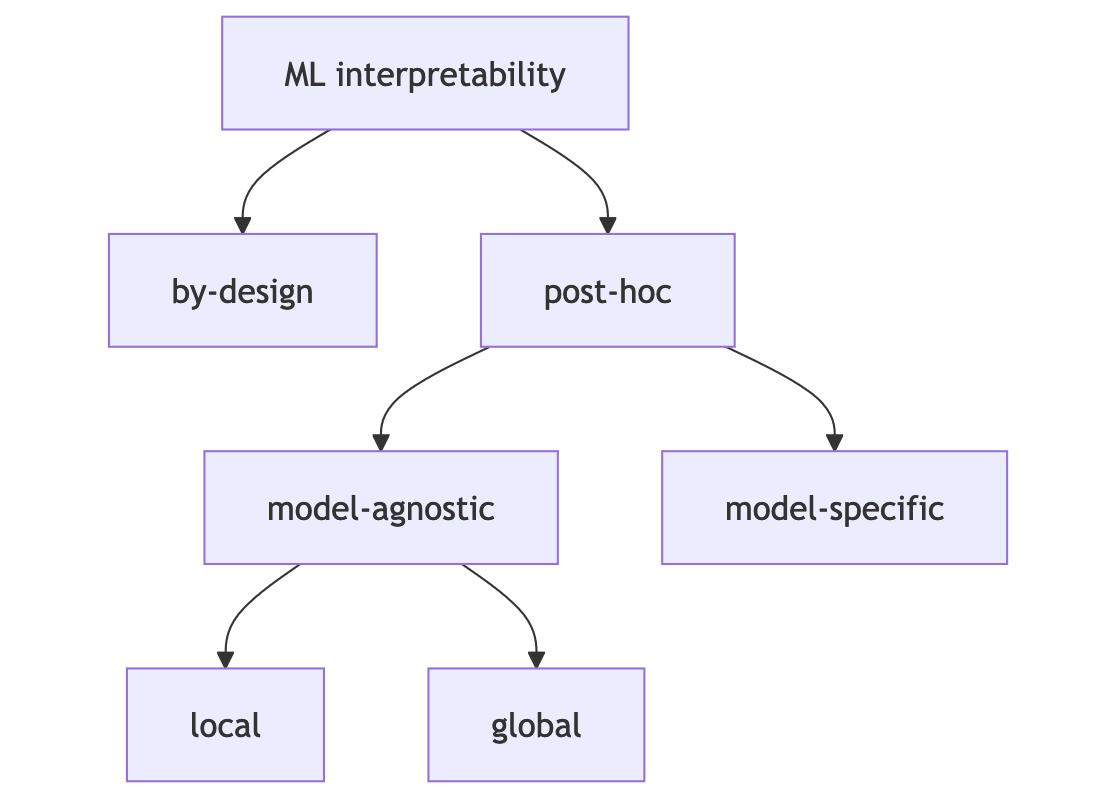
\includegraphics[width=0.8\textwidth]{../figures/static/xai-taxonomy.jpg}
    \caption{\acrshort{xai} Taxonomy \citep{Molnar2025}}
    \label{fig:xai-taxonomy}
\end{figure}

Inherently interpretable models are designed to be transparent by construction, often using simpler architectures or feature-based approaches that allow for direct interpretation of the relationship between inputs and outputs. Examples include linear regression, decision trees, and rule-based systems. A clear disadvantage is that these simpler models may sacrifice some predictive performance compared to more complex ones like \acrfull{dnn}. \acrshort{piml} could also be considered a part of this landscape, as it aims to integrate existing physical knowledge into architectures and training processes to enhance forecast accuracy and credibility. Post-hoc explanation methods, on the other hand, are applied to models after training to partially interpret their behaviour. Model-specific post-hoc methods leverage the learned structure of the model. Feature importance, as mentioned above, serves as a illustrative example, where the decision-tree model structure is integrated directly into the explanation algorithm. Notably for this research, model-agnostic methods are predominantly designed to make no assumptions about a model's underlying architecture. These methods can then be broadly categorised into local and global explanations. Local explanations focus on providing insights into model behaviour around a given input. In contrast, global explanations aim to provide an overall understanding of the model's behaviour for any input. For local explanations, counterfactual analysis has gained traction, especially for classification tasks, where the model's local decision boundary can be more interactively explored through slight perturbations of the a given input \citep{Mothilal2019}. \acrfull{shap} is both applicable for local and global explanations and will be used extensively throughout this research. As such, a brief overview of the approach follows.

\subsection{Shapley Additive Explanations}

After its popularisation via \cite{Lundberg2017} and the accompanying \texttt{shap} \texttt{python} library, \acrfull{shap} has emerged as one of the most prominent frameworks for post-hoc explainability. This is achieved through the application of coalitional game theory where the algorithm approximates a fair distribution of "payout", in this case a fraction of the model's prediction, among the input features based on their individual contributions to the prediction \citep{Shapley1953}. Formally, the Shapley value for a feature is calculated via the average marginal contribution of that feature across all possible coalitions of features weighted by the probability of the coalition, where a coalition is a subset of features, and the marginal contribution of a feature to a coalition is the difference in the model's prediction when that feature is included versus when it is excluded. This process ensures that each feature's contribution is fairly evaluated by accounting for its interactions with other features. The result is a set of Shapley values for each feature and model output, which can then be used to interpret the model's predictions locally, by highlighting the most influential features for a single output, or globally, by aggregating the Shapley values across multiple predictions to identify overall feature importance.

In practice, this algorithm experiences a \gls{combinatorialexplosion} as features increase, thus, various approximations and optimisations have been developed to make it feasible for larger datasets. For example, \cite{Lundberg2017} present a kernel-based method which operates on the assumption that not all coalitions are equally important in quantifying a features marginal contribution. The application of Shapley values for explaining \acrshort{ml} models was first proposed by \cite{trumbelj2011}, but \cite{Lundberg2017} key contribution was the introduction of an additive feature attribution model, which allows for efficient approximation using a linear model. This approach assumes that the prediction can be expressed as a sum of the feature contributions, making it easier to interpret and visualise. The \texttt{shap} library implements both model-specific and agnostic methods using this framework and provides various tools for visualising Shapley values and their impact on individual predictions and overall model performance.

\begin{itemize}
    \item use shap values to identify key features driving model predictions
\end{itemize}

\subsection{Geographic and Temporal Distribution of Feature Importance}

\begin{itemize}
    \item find highest correlation (or other relation measure) of shap values to lon, lat, eat hours, and date angle to analyse feature importance across different regions and time periods
\end{itemize}